\subsection{Sleep Stage Detection via Respiration Signal}
Identifying change points in real-world data is challenging due to cyclic, seasonal, and environmental effects. In this context, we use a dataset of respiration signals from a sleep stage detection task. The datasets represent respiration (thorax extension), sampled at 10 Hz from different subjects. The data are manually labeled by Dr.~J. Rittweger from the Institute for Physiology at the Free University of Berlin. For details, refer to the original publication~\cite{Keogh2005}. For comparison with online SVD, we use the same hyperparameters as in the previous section, listed in Table~\ref{table:kawahara_comp_hyperparameters}.

\paragraph{NPRS43}
The comparison results of experiments conducted on the NPRS43 dataset are presented in Figure~\ref{fig:nprs43}. This dataset spans approximately 7 minutes of sleep respiration signals of a subject. The subject is in stage II deep sleep for the first 5 minutes, then transitions through a short awake stage of approximately 1 minute to the stage I sleep. The transitions are marked as red vertical lines in the plot. Due to the size of the test set, the peak of change-point statistics is delayed by \(c\) snapshots and marked as red dashed vertical lines.

Both methods identify the first transition from stage II to the awake state with a peak of statistics delayed by \(c\). While SVD fails to recognize the second transition, our method displays an increased score with significant delay after the transition. Since the delay is longer than \(a + c\), it could be regarded as a false positive (FP) detection of a change point. Nonetheless, by visually examining data after the ground truth label, it could be argued that the second transition occurs more gradually and spans multiple breathing cycles, two with very short thrax extensions after the ground truth label, followed by two with larger thrax extensions and ended by two very large extensions. Our method seems to capture the middle point of this gradual transition as a reference, and learning windows cross the first transition point. The validity of this reasoning was not supported by the

\begin{figure}
	\centering
	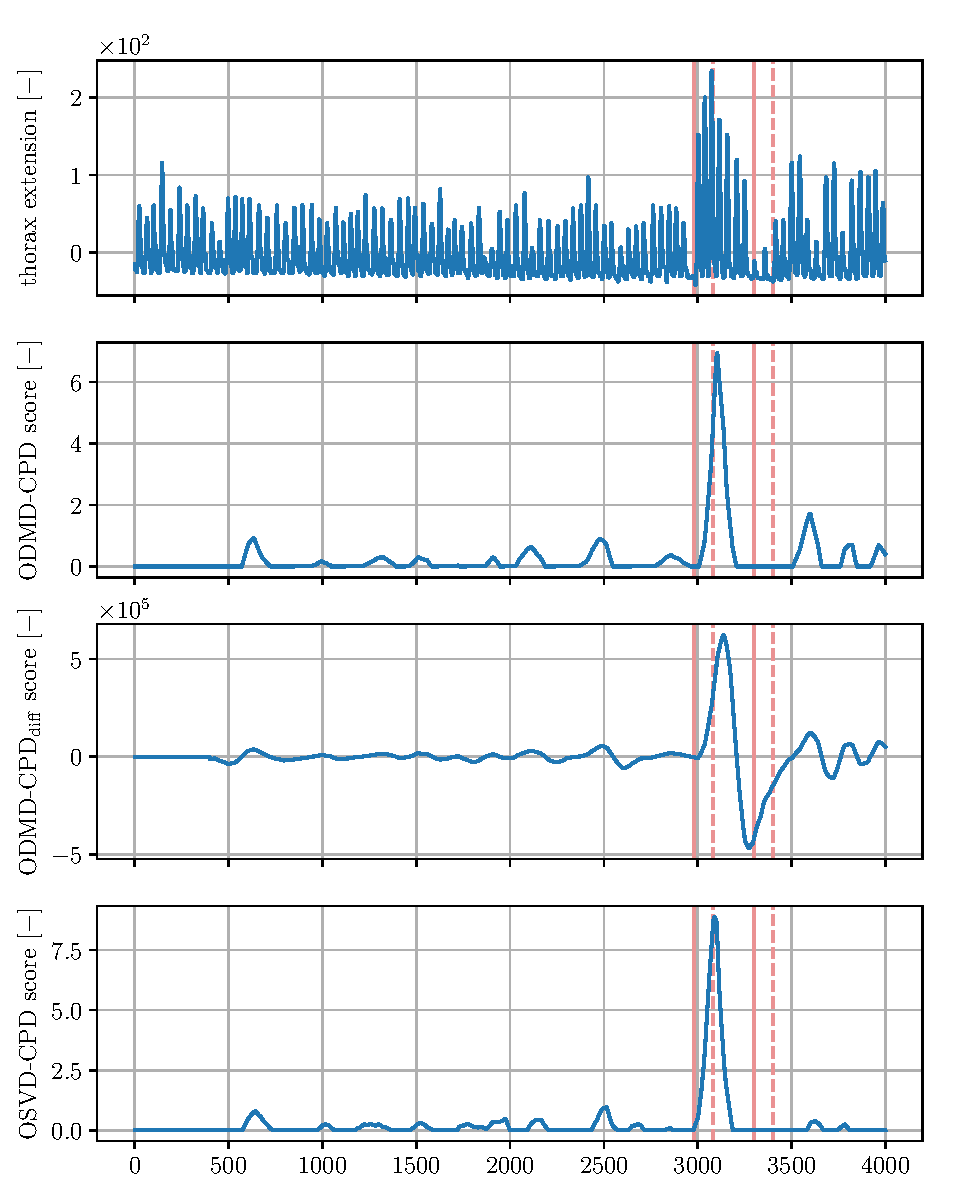
\includegraphics[width=\linewidth]{figures/nprs43-chd_r2-roll_301-dmd_w1.0-h80.pdf}
	\caption{NPRS43: Sleep stage transition detection based on respiration data (1). Change score is evaluated for the proposed method as presented in Section~\ref{sec:method} (2), the proposed method evaluating score as the difference of errors (3), and the reference method using online SVD (4). While both methods detect the first CP, our method detects the second CP as well, albeit with a longer delay due to the proximity of the CPs.}\label{fig:nprs43}
\end{figure}

\paragraph{NPRS44}
The comparison results of experiments conducted on the NPRS44 dataset are presented in Figure~\ref{fig:nprs44}. This dataset spans approximately 11 minutes of sleep respiration signals of a subject. The subject is in stage II deep sleep for the first 4 minutes, then transitions through the stage I sleep, indicated by shallow breathing, for approximately 4 minutes to an awake state. The transitions are marked as red vertical lines, and the ideal change statistics peak as grey lines in the plot.

Both methods identify the transitions present in the dataset with high discrimination capacity. CPD-DMD has significantly fewer sharp peaks in areas where a transition is not anticipated compared to the SVD-based method. Moreover, CPD-DMD captures the second transition with higher prominence and achieves peak detection with a delay of exactly \(c\) snapshots. Under the same parametrization, CPD-DMD shows smoother scores and slightly better discrimination of the transitions.

\begin{figure}[H]
	\centering
	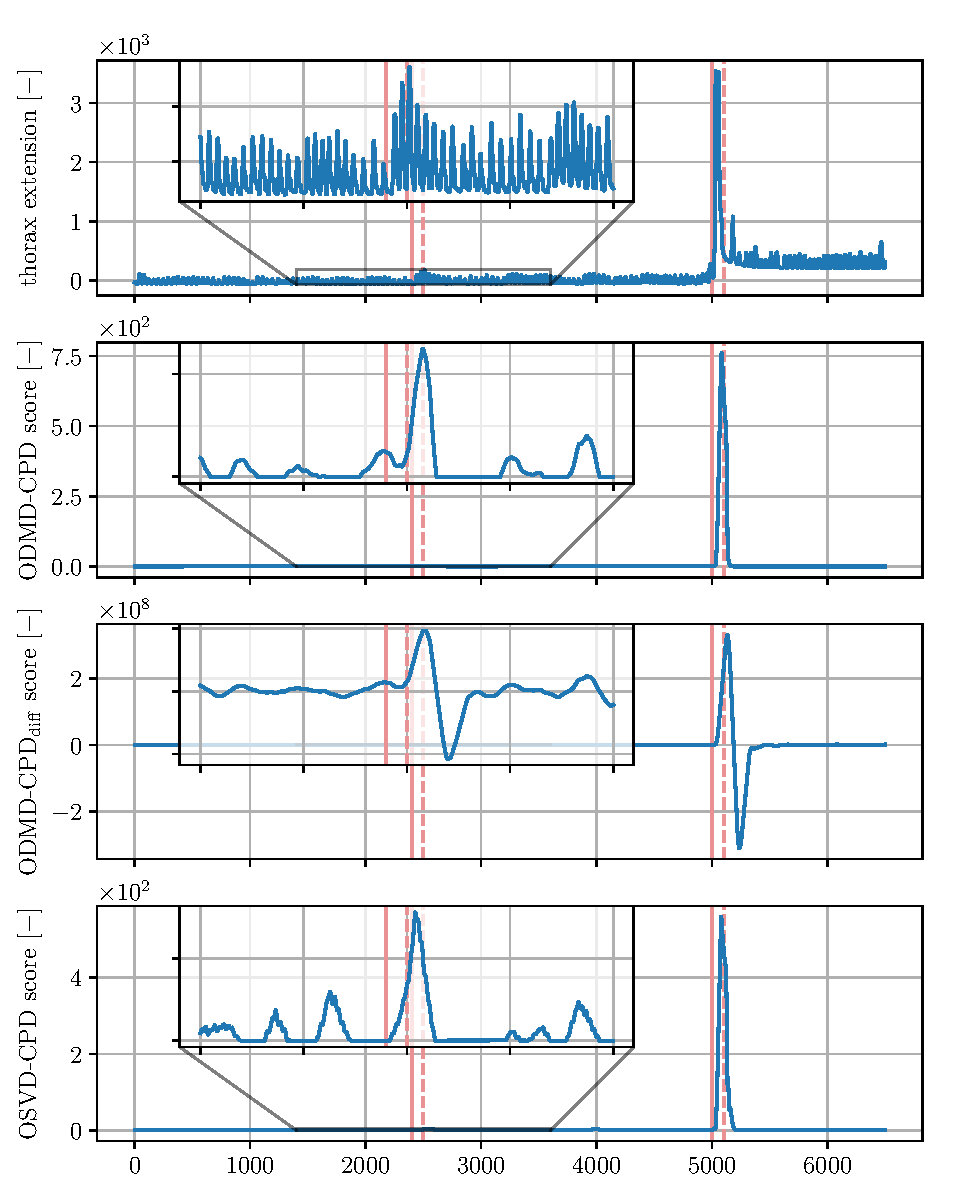
\includegraphics[width=\linewidth]{figures/nprs44-chd_r2-roll_301-dmd_w1.0-h80.pdf}
	\caption{NPRS434: Sleep stage transition detection based on respiration data (1). Change score is evaluated for the proposed method as presented in Section~\ref{sec:method} (2), the proposed method evaluating score as the difference of errors (3), and the reference method using online SVD (4). While both methods detect CPs, our method detects the first one with a score three times higher than the peaks unrelated to tracked events, while OSVD only doubles the score.}\label{fig:nprs44}
\end{figure}
